% Created by tikzDevice version 0.12.3.1 on 2022-09-05 10:53:56
% !TEX encoding = UTF-8 Unicode
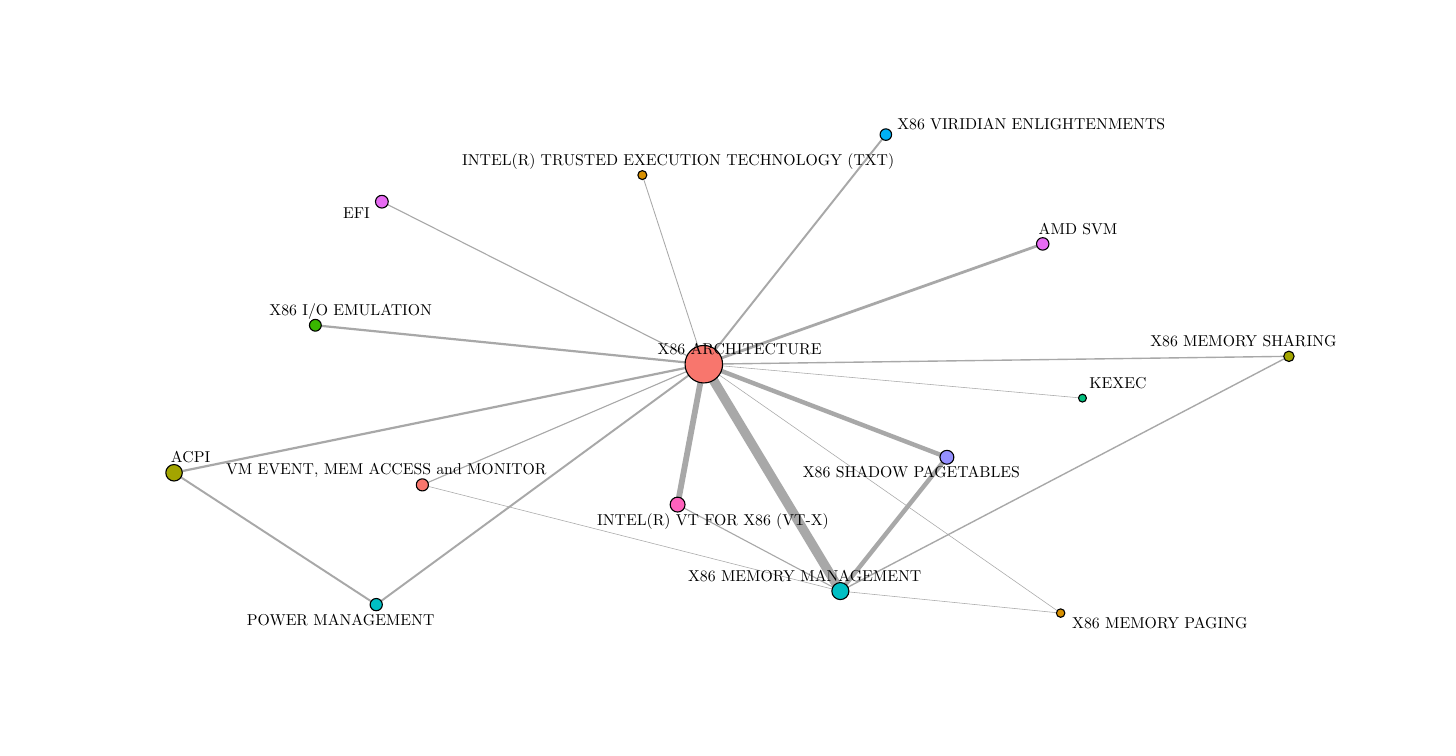
\begin{tikzpicture}[x=1pt,y=1pt]
\definecolor{fillColor}{RGB}{255,255,255}
\path[use as bounding box,fill=fillColor,fill opacity=0.00] (0,0) rectangle (505.89,252.94);
\begin{scope}
\path[clip] (  0.00,  0.00) rectangle (505.89,252.94);
\definecolor{fillColor}{RGB}{255,255,255}

\path[fill=fillColor] (  0.00,  0.00) rectangle (505.89,252.94);
\end{scope}
\begin{scope}
\path[clip] ( 32.75, 32.75) rectangle (475.89,222.94);
\definecolor{drawColor}{gray}{0.66}

\path[draw=drawColor,line width= 0.7pt,line join=round] ( 52.89, 92.10) -- (125.95, 44.46);

\path[draw=drawColor,line width= 0.8pt,line join=round] ( 52.89, 92.10) -- (244.32,131.33);

\path[draw=drawColor,line width= 1.0pt,line join=round] (366.79,174.80) -- (244.32,131.33);

\path[draw=drawColor,line width= 0.4pt,line join=round] (127.99,190.06) -- (244.32,131.33);

\path[draw=drawColor,line width= 0.3pt,line join=round] (222.11,199.67) -- (244.32,131.33);

\path[draw=drawColor,line width= 2.1pt,line join=round] (234.85, 80.60) -- (244.32,131.33);

\path[draw=drawColor,line width= 0.4pt,line join=round] (234.85, 80.60) -- (293.66, 49.35);

\path[draw=drawColor,line width= 0.2pt,line join=round] (381.15,119.08) -- (244.32,131.33);

\path[draw=drawColor,line width= 0.7pt,line join=round] (125.95, 44.46) -- (244.32,131.33);

\path[draw=drawColor,line width= 0.4pt,line join=round] (142.62, 87.73) -- (244.32,131.33);

\path[draw=drawColor,line width= 0.2pt,line join=round] (142.62, 87.73) -- (293.66, 49.35);

\path[draw=drawColor,line width= 0.8pt,line join=round] (244.32,131.33) -- (103.95,145.40);

\path[draw=drawColor,line width= 3.4pt,line join=round] (244.32,131.33) -- (293.66, 49.35);

\path[draw=drawColor,line width= 0.2pt,line join=round] (244.32,131.33) -- (373.26, 41.40);

\path[draw=drawColor,line width= 0.5pt,line join=round] (244.32,131.33) -- (455.75,134.18);

\path[draw=drawColor,line width= 1.6pt,line join=round] (244.32,131.33) -- (332.16, 97.70);

\path[draw=drawColor,line width= 0.7pt,line join=round] (244.32,131.33) -- (310.10,214.30);

\path[draw=drawColor,line width= 0.2pt,line join=round] (293.66, 49.35) -- (373.26, 41.40);

\path[draw=drawColor,line width= 0.5pt,line join=round] (293.66, 49.35) -- (455.75,134.18);

\path[draw=drawColor,line width= 1.6pt,line join=round] (293.66, 49.35) -- (332.16, 97.70);
\definecolor{drawColor}{RGB}{0,0,0}
\definecolor{fillColor}{RGB}{163,165,0}

\path[draw=drawColor,line width= 0.4pt,line join=round,line cap=round,fill=fillColor] ( 52.89, 92.10) circle (  2.98);
\definecolor{fillColor}{RGB}{231,107,243}

\path[draw=drawColor,line width= 0.4pt,line join=round,line cap=round,fill=fillColor] (366.79,174.80) circle (  2.25);

\path[draw=drawColor,line width= 0.4pt,line join=round,line cap=round,fill=fillColor] (127.99,190.06) circle (  2.30);
\definecolor{fillColor}{RGB}{216,144,0}

\path[draw=drawColor,line width= 0.4pt,line join=round,line cap=round,fill=fillColor] (222.11,199.67) circle (  1.62);
\definecolor{fillColor}{RGB}{255,98,188}

\path[draw=drawColor,line width= 0.4pt,line join=round,line cap=round,fill=fillColor] (234.85, 80.60) circle (  2.69);
\definecolor{fillColor}{RGB}{0,191,125}

\path[draw=drawColor,line width= 0.4pt,line join=round,line cap=round,fill=fillColor] (381.15,119.08) circle (  1.43);
\definecolor{fillColor}{RGB}{0,191,196}

\path[draw=drawColor,line width= 0.4pt,line join=round,line cap=round,fill=fillColor] (125.95, 44.46) circle (  2.21);
\definecolor{fillColor}{RGB}{248,118,109}

\path[draw=drawColor,line width= 0.4pt,line join=round,line cap=round,fill=fillColor] (142.62, 87.73) circle (  2.19);

\path[draw=drawColor,line width= 0.4pt,line join=round,line cap=round,fill=fillColor] (244.32,131.33) circle (  6.78);
\definecolor{fillColor}{RGB}{57,182,0}

\path[draw=drawColor,line width= 0.4pt,line join=round,line cap=round,fill=fillColor] (103.95,145.40) circle (  2.13);
\definecolor{fillColor}{RGB}{0,191,196}

\path[draw=drawColor,line width= 0.4pt,line join=round,line cap=round,fill=fillColor] (293.66, 49.35) circle (  3.08);
\definecolor{fillColor}{RGB}{216,144,0}

\path[draw=drawColor,line width= 0.4pt,line join=round,line cap=round,fill=fillColor] (373.26, 41.40) circle (  1.53);
\definecolor{fillColor}{RGB}{163,165,0}

\path[draw=drawColor,line width= 0.4pt,line join=round,line cap=round,fill=fillColor] (455.75,134.18) circle (  1.88);
\definecolor{fillColor}{RGB}{149,144,255}

\path[draw=drawColor,line width= 0.4pt,line join=round,line cap=round,fill=fillColor] (332.16, 97.70) circle (  2.51);
\definecolor{fillColor}{RGB}{0,176,246}

\path[draw=drawColor,line width= 0.4pt,line join=round,line cap=round,fill=fillColor] (310.10,214.30) circle (  2.08);

\node[text=drawColor,anchor=base,inner sep=0pt, outer sep=0pt, scale=  0.57] at ( 58.87, 95.71) {ACPI};

\node[text=drawColor,anchor=base,inner sep=0pt, outer sep=0pt, scale=  0.57] at (379.56,178.35) {AMD SVM};

\node[text=drawColor,anchor=base,inner sep=0pt, outer sep=0pt, scale=  0.57] at (118.78,184.15) {EFI};

\node[text=drawColor,anchor=base,inner sep=0pt, outer sep=0pt, scale=  0.57] at (235.06,203.23) {INTEL(R) TRUSTED EXECUTION TECHNOLOGY (TXT)};

\node[text=drawColor,anchor=base,inner sep=0pt, outer sep=0pt, scale=  0.57] at (247.63, 73.13) {INTEL(R) VT FOR X86 (VT-X)};

\node[text=drawColor,anchor=base,inner sep=0pt, outer sep=0pt, scale=  0.57] at (393.97,122.63) {KEXEC};

\node[text=drawColor,anchor=base,inner sep=0pt, outer sep=0pt, scale=  0.57] at (113.11, 36.98) {POWER MANAGEMENT};

\node[text=drawColor,anchor=base,inner sep=0pt, outer sep=0pt, scale=  0.57] at (129.59, 91.36) {VM EVENT, MEM ACCESS and MONITOR};

\node[text=drawColor,anchor=base,inner sep=0pt, outer sep=0pt, scale=  0.57] at (257.26,134.93) {X86 ARCHITECTURE};

\node[text=drawColor,anchor=base,inner sep=0pt, outer sep=0pt, scale=  0.57] at (116.75,148.94) {X86 I/O EMULATION};

\node[text=drawColor,anchor=base,inner sep=0pt, outer sep=0pt, scale=  0.57] at (280.80, 52.93) {X86 MEMORY MANAGEMENT};

\node[text=drawColor,anchor=base,inner sep=0pt, outer sep=0pt, scale=  0.57] at (409.12, 35.76) {X86 MEMORY PAGING};

\node[text=drawColor,anchor=base,inner sep=0pt, outer sep=0pt, scale=  0.57] at (439.31,137.74) {X86 MEMORY SHARING};

\node[text=drawColor,anchor=base,inner sep=0pt, outer sep=0pt, scale=  0.57] at (319.34, 90.23) {X86 SHADOW PAGETABLES};

\node[text=drawColor,anchor=base,inner sep=0pt, outer sep=0pt, scale=  0.57] at (362.65,216.01) {X86 VIRIDIAN ENLIGHTENMENTS};
\end{scope}
\end{tikzpicture}
